\section{Bi-orthogonal Bases}\label{sec: bi-orth}
In this section, we analyze bi-orthogonal bases in the following form of MRA,
\begin{align}\label{eq: bi-orth MRA}
\{\phi_{L,\V{k}},\widetilde{\phi}_{L,\V{k}}, \psi_{l,\V{k}'}^j,\widetilde{\psi}_{l,\V{k}'}^j,\, 1\leq l\leq L,\,\V{k}\in\mathbb{Z}^2,\, \V{k}'\in\mathbf{Q}\mathbb{Z}^2,\,1\leq j\leq J \},
\end{align}
where $\phi$ and $\psi^j$ satisfy \eqref{eq: m0} and \eqref{eq: mj}, as well as $\widetilde{\phi}$ and $\widetilde{\psi^j}$, respectively,
$$\widehat{\widetilde{\phi}}(\V{D}^T\V{\omega}) = \widetilde{m_0}(\V{\omega})\widehat{\widetilde{\phi}}(\V{\omega}),\quad \widehat{\widetilde{\psi^j}}(\V{D}^T\V{\omega}) = \widetilde{m_j}(\V{\omega})\widehat{\widetilde{\phi}}(\V{\omega}).$$
For bi-orthogonal bases, we have the similar identity summation and shift cancellation condition to those in Theorem \ref{thm: conds}.
\begin{thm}\label{thm: bi-orth conds}
The perfect reconstruction iff the following two conditions hold
\begin{align}\label{eq: id-sum 2}
m_0(\boldsymbol{\omega})\sbarm{0} + \sum_{j = 1}^6 m_j(\boldsymbol{\omega})\sbarm{j} = 1
\end{align}
\begin{equation}\label{eq: shift-cancel 2}
\begin{cases}
\sum_{j = 0}^6m_j(\boldsymbol{\omega})\overline{\widetilde{m_j}}(\boldsymbol{\omega} + \boldsymbol{\pi}) = 0, & \boldsymbol{\pi}\in \Gamma_0\setminus\{\boldsymbol{0}\}\\[.5em]
\sum_{j=1}^6m_j(\boldsymbol{\omega})\overline{\widetilde{m_j}}(\boldsymbol{\omega}+\boldsymbol{\pi}) = 0, & \boldsymbol{\pi}\in\Gamma_1\setminus\Gamma_0
\end{cases}
\end{equation}
\end{thm}
The conditions \eqref{eq: id-sum 2} and \eqref{eq: shift-cancel 2} can be combined into a linear system as follows,
\begin{align}\label{eq: LS-new}
%\overline{\M}(\V{\omega})\mathbf{m}_0(\V{\omega})=
\begin{bmatrix}
    \,\sbarm{0} & \sbarm{1} & \hdots & \sbarm{6}\;  \\
    \;0 & \sbarmp{1}{1}  & \hdots  & \sbarmp{6}{1}\; \\
    \,\sbarmp{0}{2} & \sbarmp{1}{2} & \hdots & \sbarmp{6}{2}\;\\
    \;\vdots & \vdots & \vdots & \vdots \; \\
    \;0 & \sbarmp{1}{7} & \hdots & \sbarmp{6}{7}\;
\end{bmatrix}
\begin{bmatrix}
\;\mo{0}\; \\
\;\mo{1}\; \\
\;\mo{2}\; \\
\; \vdots\; \\
\;\mo{6}\; 
\end{bmatrix} 
=
\begin{bmatrix}
1\\
0\\
0\\
\vdots \\
0
\end{bmatrix}
\end{align}
%where $\M\in\mathbb{C}^{8\times 7}$ and $\mathbf{m}_0\in\mathbb{C}^7$.
In addition, we have the following condition when \eqref{eq: bi-orth MRA} is bi-orthogonal, an analogue of Theorem \ref{thm: basis cond}.
\begin{thm}\label{thm: basis cond 2}
Assume that $m_0, \widetilde{m_0}$ are trigonometric polynomials with $m_0(0)=\widetilde{m_0}(0) = 1$, which generate $\phi,\widetilde{\phi}$ respectively.\\
If $\phi(\cdot - \boldsymbol{k}),\widetilde{\phi}(\cdot - \boldsymbol{k})\boldsymbol{k}\in\mathbb{Z}^2$ are bi-orthogonal, then $\exists K$ containing a neighborhood of 0, s.t. $\forall\boldsymbol{\omega}\in S_0,\,\boldsymbol{\omega}+2\pi\mathbf{n}\in K$ for some $\mathbf{n}\in\mathbb{Z}^2, $ and $\inf_{k>0,\,\boldsymbol{\omega}\in K}|m_0(\mathbf{D_2}^{-k}\boldsymbol{\omega})| >0$, $\inf_{k>0,\,\boldsymbol{\omega}\in K}|\widetilde{m_0}(\mathbf{D_2}^{-k}\boldsymbol{\omega})| >0$. 
 Further, if  $\sum_{\boldsymbol{\V{\pi}}\in \Gamma_0} m_0(\boldsymbol{\omega}+\boldsymbol{\pi})\sbarmp{0}{} = 1,$ then the inverse is true.
\end{thm}
By Theorem \ref{thm: basis cond 2}, the linear system \eqref{eq: LS-new} of a bi-orthogonal basis need to satisfy the following identity constraint on $m_0$ and $\widetilde{m_0}$,
\begin{align}\label{eq: identity-cond}
m_0\sbarm{0} + m_0\sbarmp{0}{2} + m_0\sbarmp{0}{4} + m_0\sbarmp{0}{6} = 1.
\end{align}
We thus consider feasible solutions of \eqref{eq: LS-new} with constraint \eqref{eq: identity-cond} using the same approach in \cite{cohen1993compactly}, which solves compactly supported symmetric bi-orthogonal filters on hexagon lattice. We next review the main scheme in \cite{cohen1993compactly} and extend it to our setup of directional wavelet filter.

\subsection{Summary of Cohen et al's construction}\label{subsec: cohen-summary}
We summerize the main setup and the approach in \cite{cohen1993compactly}. Consider a bi-orthogonal scheme consists of 3 high-pass filters $m_1,m_2$ and $m_3$ and a low-pass filter $m_0$ together with their bi-orthogonal duals $\widetilde{m_j}$, s.t.
$m_0$ is $\frac{2\pi}{3}$-rotation invariant and $m_1,\, m_2,\, m_3$ are $\frac{2\pi}{3}$-rotation co-variant.

This bi-orthogonal scheme satisfies the following linear system (
Lemma 2.2.2 in \cite{cohen1993compactly} )
\begin{align}\label{eq: LS}
\begin{bmatrix}
    \,\barm{0} & \barm{1} & \barm{2} & \barm{3}\;  \\
    \;\barmn{0}{1} & \barmn{1}{1}  & \barmn{2}{1}  & \barmn{3}{1}\; \\
    \;\vdots & \vdots & \vdots & \vdots \; \\
    \;\barmn{0}{3} & \barmp{1}{3} & \barmn{2}{3} & \barmn{3}{3}\;
\end{bmatrix}
\begin{bmatrix}
\;\mo{0}\; \\
\;\mo{1}\; \\
\;\mo{2}\; \\
\;\mo{3}\; 
\end{bmatrix} 
=
\begin{bmatrix}
1\\
0\\
0\\
0
\end{bmatrix}
\end{align}
 or equivalently \(\widetilde{\mathbf{M}}\, \mathbf{m} = [1,0,0,0]^\top\), where $\widetilde{\mathbf{M}}\in\mathbb{C}^{4\times 4}$ and $\V{\nu}_1 = (\pi,0),\V{\nu}_2 = (0,\pi),\V{\nu}_3=(\pi,\pi)$.\\
Given $\m{1}$, which by symmetry defines $\m{2},\,\m{3}$, we can compute $m_0$, 
\begin{align}\label{eq: m0-sol}
m_0(\V{\omega}) &= D^{-1}%\propto 
\left|
\begin{matrix}
    \; \sbarmn{1}{1}  & \sbarmn{2}{1}  & \sbarmn{3}{1}\; \\
    \; \sbarmn{1}{2}  & \sbarmn{2}{2}  & \sbarmn{3}{2}\; \\
    \; \sbarmn{1}{3} & \sbarmn{2}{3} & \sbarmn{3}{3}\;
\end{matrix}
\right| \notag\\
&= D^{-1}\det(\widetilde{\mathbf{M}}_{1,1}(\V{\omega})), \, D\in \mathbb{R}^+
\end{align}
if $\widetilde{\mathbf{M}}$ is invertible; both $\mo{0}$ and $\det(\widetilde{\mathbf{M}}_{1,1}(\V{\omega}))$, the minor of $\widetilde{\mathbf{M}}$ associated with $\sbarm{0}$, have invariance by $\frac{2\pi}{3}$.\\
{\it Remark.} For \eqref{eq: m0-sol} to hold, $\mo{0}$ and $\det(\widetilde{\mathbf{M}}_{1,1}(\V{\omega}))$ having the same phase suffices. \\
If $\widetilde{m_0}$ is solved, then $m_1,m_2$ and $m_3$ are obtained by solving the linear system \eqref{eq: LS}.
To get $\m{0}$, we solve 
\begin{align}\label{eq: bi-orth-eq}
m_0\sbarm{0} + m_0\sbarmn{0}{1} + m_0\sbarmn{0}{2} + m_0\sbarmn{0}{3} = 1
\end{align}
from expanding $det(\widetilde{\mathbf{M}})$ with respect to the first column.
According to Lemma 3.2.1 in \cite{cohen1993compactly} based on {\it Hilbert's Nullstellensatz}, \eqref{eq: bi-orth-eq} has a solution iff there does not exist $(z_1,z_2)\in (\mathbb{C}^*)^2,\, \mathbb{C}^* = \mathbb{C}\setminus\{0\}$ s.t. $(\pm z_1,\pm z_2)$ are four 
vanishing points of the $z$-transform of $m_0$.

\subsubsection{Solving $\m{0}$}
In general, there is no efficient algorithm to solve {\it Hilbert's Nullstellensatz}, and how \eqref{eq: identity-cond} is solved exactly is not mentioned in \cite{cohen1993compactly}.

We propose an optimization approach, where \eqref{eq: identity-cond} is equivalent to a linear constraint and the objective function imposes regularity on $\widetilde{m_0}$.
On a $2N\times 2N$ grid $\G$ of $S_0 = [-\pi, \pi)\times[-\pi, \pi)$, s.t. $\forall \V{\omega}_j \in \G, \; \V{\omega}_j+\V{\nu}_1,\,\V{\omega}_j+\V{\nu}_2,\,\V{\omega}_j+\V{\nu}_3 \in \G$, \eqref{eq: identity-cond} is reformulated as
\begin{align}
\hspace*{10em} \V{A}\, \mathbf{\widetilde{m}_0}&= \mathbf{1}_{4N^2}, \label{eq: m0-A}\\ 
\mathbf{\widetilde{m}_0} = [\widetilde{m_0}(\V{\omega}_i)]_{\,i=1,\hdots,4N^2} \quad &\V{A}_{i,j} = m_0(\V{\omega}_j)\sum_{k=0}^3\delta(\V{\omega}_j-\V{\omega}_i-\V{\nu}_k) \notag
\end{align}
Because the set $\{\V{\omega}+\V{\nu}_k,k=0,1,2,3\}$ is invariant under the shift $\V{\nu}_i,\, i = 1,2,3,$ the rows of $\V{A}$ corresponding to $\V{\omega}$ and $\V{\omega}+\V{\nu}_i$ are identical and we only need to consider rows corresponds to $\V{\omega}\in [-\pi,\pi)\times[-\pi,\pi)/\{\V{\nu}_i,i=0,1,2,3\}$. Therefore, after removing the duplicate rows, $\V{A}\in \mathbb{C}^{N^2\times 4N^2}$ and \eqref{eq: m0-A} is under-determinant. \\
We thus use \eqref{eq: m0-A} as a linear constraint in quadratic optimization to solve $\mathbf{\widetilde{m}_0}$. Suppose that $\m{0}$ should is smooth, and we build a differential operator $\V{D}$ and solve the following minimization problem:
\begin{align}
&\min_{\mvec{0}}\; \Vert \V{D}\mvec{0}\Vert^2,\quad s.t. \; \V{A}\mvec{0} = \mathbf{1} \label{eq: opt-diff}
\end{align}
%or
%\begin{align}
%&\min_{\mvec{0}}\; \Vert \V{D}\mvec{0}\Vert^2 + \lambda \Vert \V{A}\mvec{0} - \mathbf{1}\Vert^2 \label{eq: m0-smooth-relaxed}
%\end{align}
%The solution of \eqref{eq: m0-smooth-relaxed} is $\mvec{0} = \lambda(\lambda \V{A}^\top \V{A} + \V{D}^\top \V{D})^{-1}\V{A}^\top\mathbf{1}$.

Or suppose $\m{0}$ decays away from the origin, then we build a diagonal weighting operator $\V{W}$, and solve the following minimization problem:
\begin{align}\label{eq: opt-weight}
&\min_{\mvec{0}}\; \Vert \V{W}\mvec{0}\Vert^2,\quad s.t. \; \V{A}\mvec{0} = \mathbf{1}
\end{align}
Supplementary numerical results on solving $\m{0}$ by optimization are provided in Appendix \ref{app: supp-numerical}, where we test this optimization method on pre-designed bi-orthogonal filters $m_0$ and $\widetilde{m_0}$.

\section{Adaptation to dilated quincunx scheme}
Following the same approach, we focus on the design of $m_i,\,i=0,\cdots,6$ and the low pass dual function $\m{0}$, given the high pass directional dual functions $\m{i},\,i=1,\cdots,6$. Assume $\m{i},\,i=1,\cdots,6$ satisfy weak constraints on the direction selectivity of their support.\\
{\bf Definition.}
The {\it essential support} $\Omega_i$ of a function $\widetilde{m_i}$ is the set $\{\V{\omega}:\,|\widetilde{m_i}(\V{\omega})|> |\widetilde{m_j}(\V{\omega})|,\,\forall j\neq i\}$. 

\begin{figure}
\centering
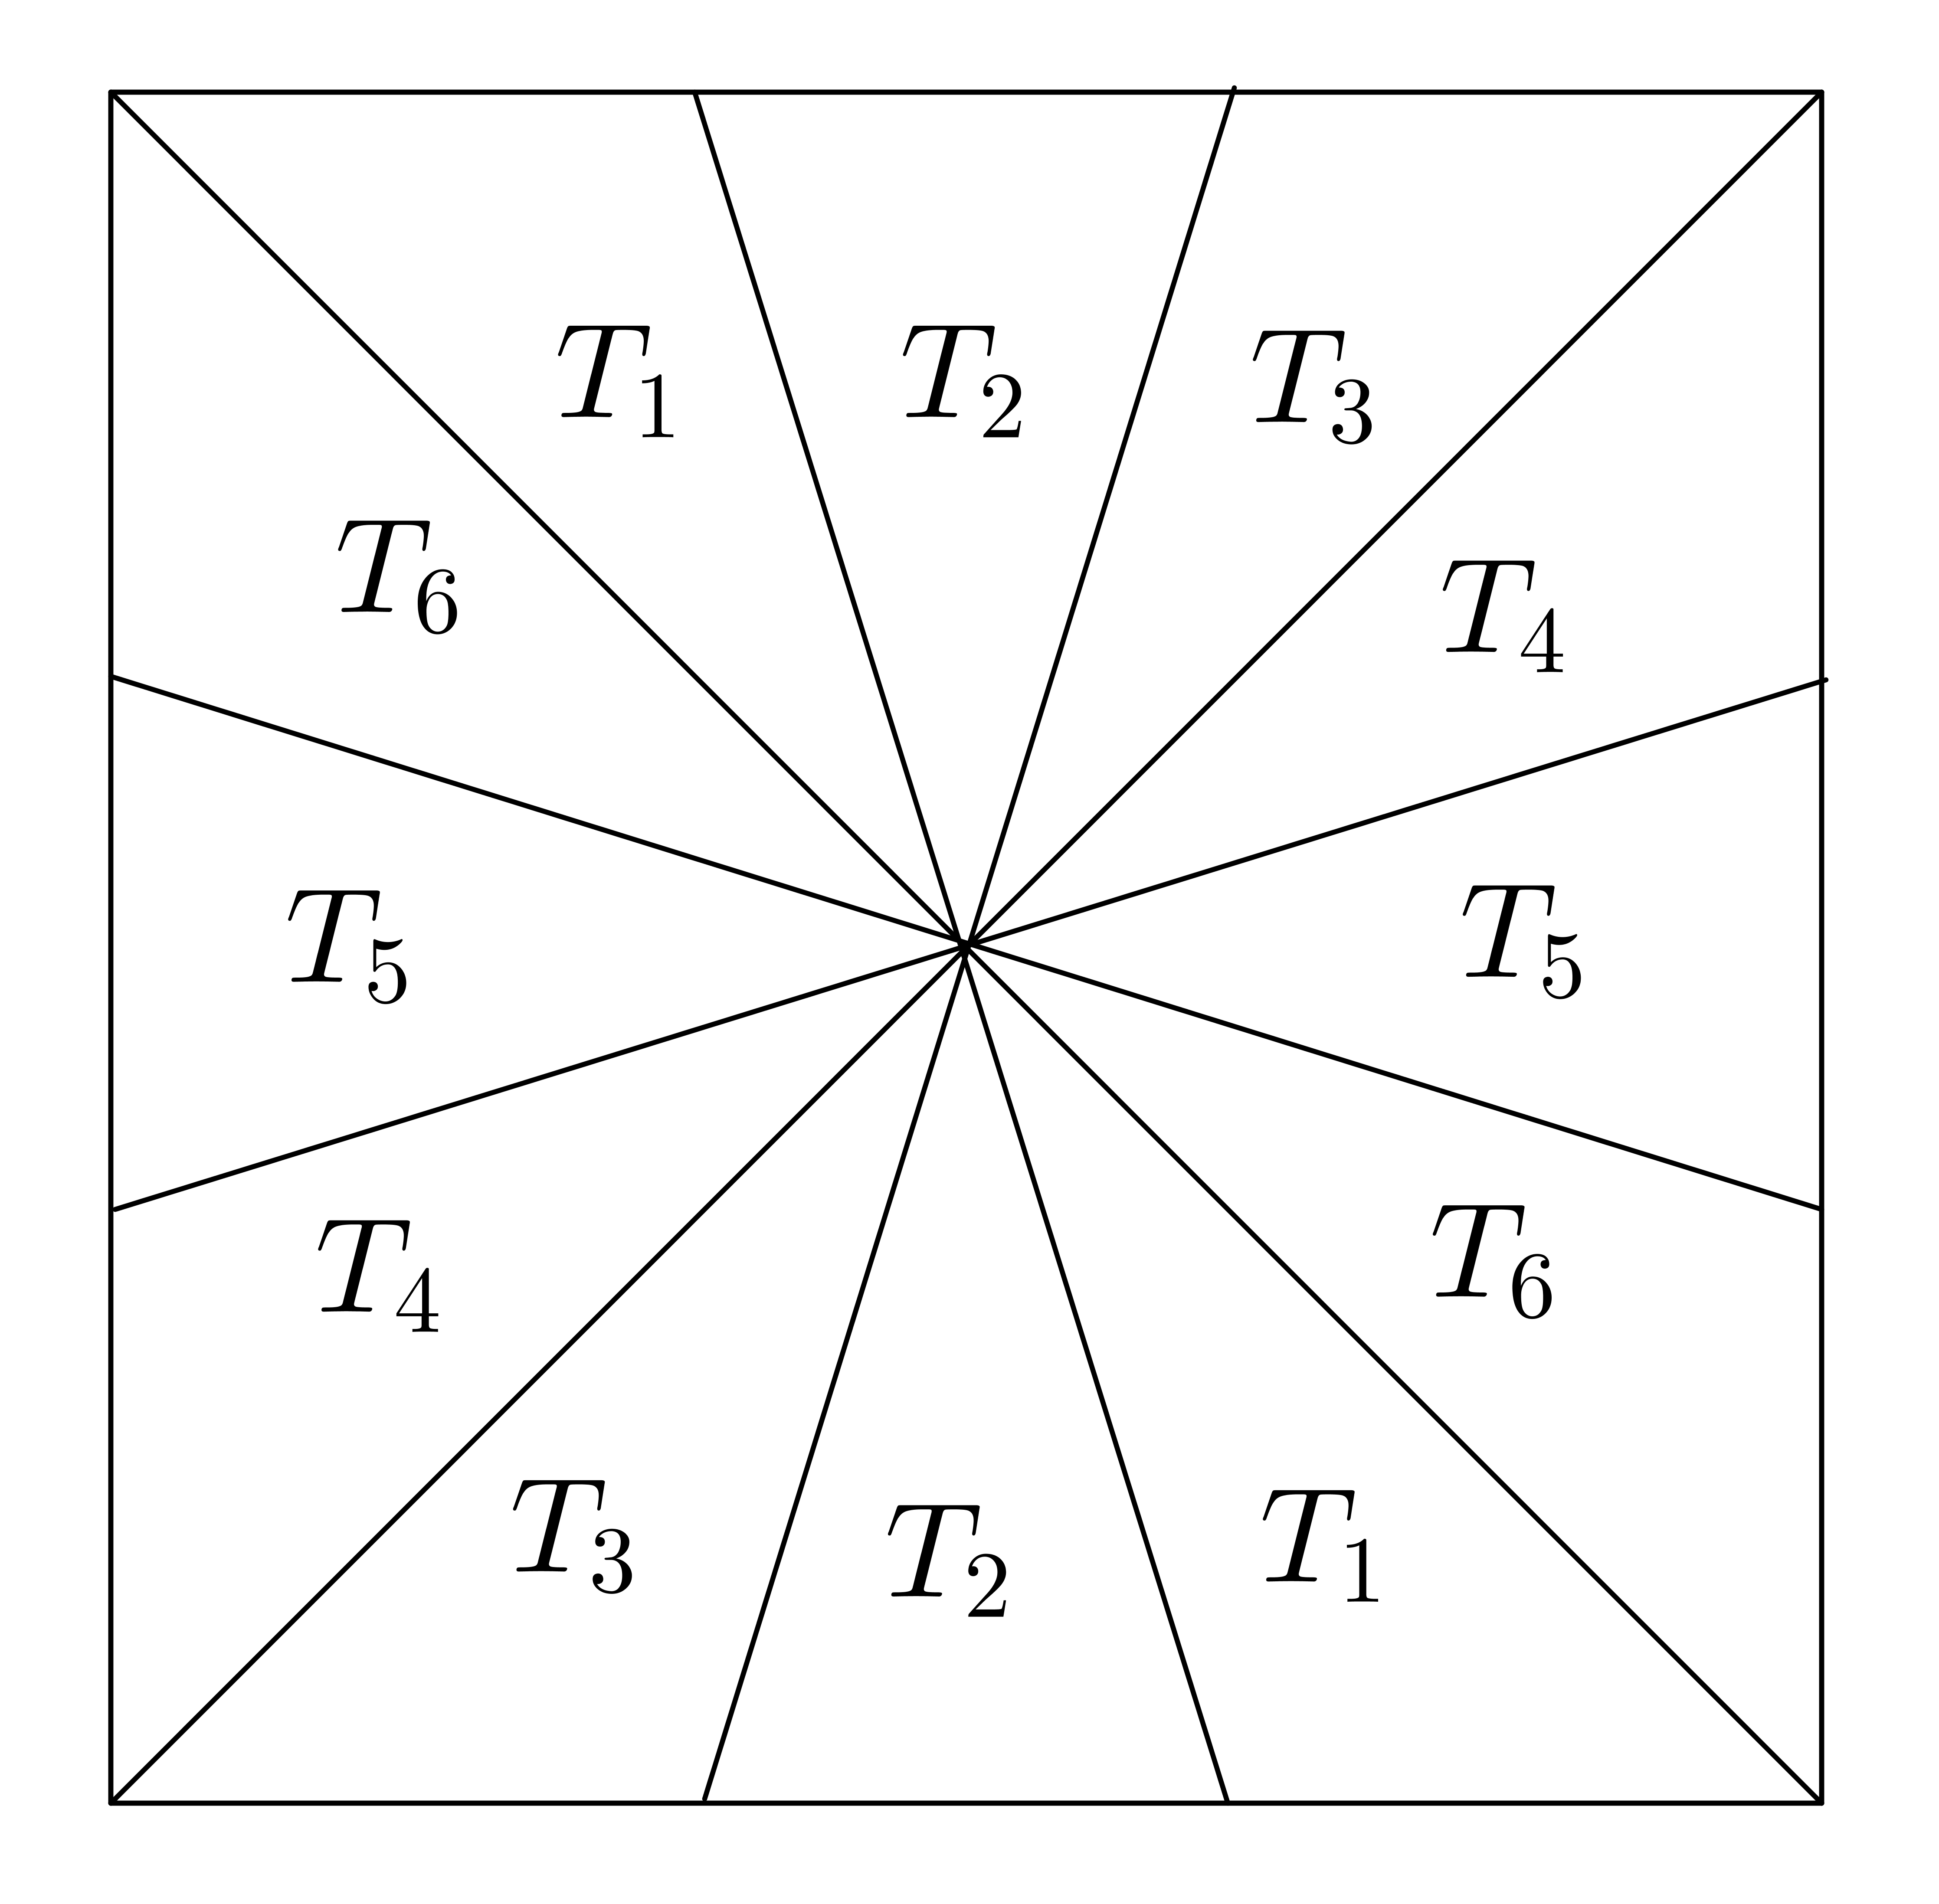
\includegraphics[width = .4\textwidth]{triangle-partition.png}
\caption{partition of frequency square in six directions, where the essential support of $\m{i}$ is contained in each pair of triangles $T_i$}
\label{fig: partition 2}
\end{figure}
Let pairs of triangles $T_i$ in Fig.\ref{fig: partition 2} contain the essential support of $\widetilde{m_i},\,i=1,\cdots,6$.
A minimum symmetry of $\m{i}$ is required such that $\m{1}$ and $\m{6}$ are symmetric with respect to the diagonal, and so are $\m{3}$ and $\m{4}$.\\
\eqref{eq: LS-new} takes a similar form to \eqref{eq: LS}, but with $\M\in\mathbb{C}^{8\times 7}$, which is an over-determinant linear system.

\subsection{Computing $m_0$}\label{subsec: compute-m0}
Same as in Section \ref{subsec: cohen-summary} , we first compute $m_0$ and assume that $\M$ is full rank, otherwise \eqref{eq: LS-new} has infinitely many solutions. Moreover, $\M[2:8,:]$ is singular. 
\begin{lemma}\label{lem: subM-singular}
$\M[2:8,:]$ is singular $\forall \V{\omega}$.
\end{lemma}
\noindent{\it Proof.}
If \eqref{eq: LS-new} has a solution, then $\forall \V{\omega}$,  $[1,0,\cdots,0]^\top$ is a linear combination of the columns of $\M$ and the solution $\mathbf{m} \in Null(\M[2:8,:])$, hence $\M[2:8,:]$ being singular is a prerequisite.\qed\\
Therefore, there is a unique row $\M[k_{\V{\omega}},:],\,k_\omega\in\{2,\cdots,8\}$ such that removing it from $\M$ gives a non-singular square matrix $\M[-k_{\V{\omega}},:]$. By Cramer's rule, $$m_0(\V{\omega}) = det(\M_{1,1}[-k_{\V{\omega}},:])/det(\M[-k_{\V{\omega}},:]),$$ where $\det(\M_{1,1}[-k_{\V{\omega}},:])$ is the minor of $\M[-k_{\V{\omega}},:]$ associated with $\m{0}$. 
Let $C_{\V{\omega}} = det(\M[-k_{\V{\omega}},:])$, then we have the following observation.
\begin{lemma}\label{lem: equal-det}
$C_{\V{\omega}} = C_{\V{\omega}+\V{\pi}_2} = C_{\V{\omega}+\V{\pi}_4} = C_{\V{\omega}+\V{\pi}_6}$
\end{lemma}
\noindent{\it Proof}
Because $\widetilde{M}(\V{\omega}+\V{\pi}_2) = P_{\V{\pi}_2}\M(\V{\omega})$ where $P_{\V{\pi}_2}$ is a row permutation matrix, it follows from the definition of $C_{\V{\omega}}$ that 
$C_{\V{\omega}} = det\big(\M[-k_{\V{\omega}},:](\V{\omega})\big) = det\big(\M[-k_{\V{\omega}+\V{\pi}_2},:](\V{\omega}+\V{\pi}_2) \big)= C_{\V{\omega}+\V{\pi}_2}$ where 
$\mathbf{1}_{k_{\V{\omega}+\V{\pi}_2}} = P_{\V{\pi}_2}\mathbf{1}_{k_{\V{\omega}}}$.
\qed\\[1em]
We assume that $m_0\in\mathbb{R}_{\geq 0}$ without phase. Let $m_0^C(\V{\omega}) = m_0(\V{\omega})|C_{\V{\omega}}|\in \mathbb{R}_{\geq 0}$ and $\mc{0} = \m{0}/|C_{\V{\omega}}|$, then Lemma \ref{lem: equal-det} implies the following.
\begin{proposition}\label{prop: mc}
$m_0(\V{\omega}),\,\m{0}, m_i(\V{\omega}),\,  i = 1,...,6$ satisfy \eqref{eq: LS-new} given $\m{i},\,i=1,...,6$ if and only if $m_0^C(\V{\omega}),$ $\,\mc{0}, m_i(\V{\omega}),\,i = 1,...,6$ do. More generally, $m_0^C(\V{\omega})c(\V{\omega}),\,\mc{0}c(\V{\omega})^{-1}, m_i(\V{\omega}),\,i=1,...,6$ satisfy \eqref{eq: LS-new} if $c(\V{\omega}) = c(\V{\omega}+\V{\pi}_2)=c(\V{\omega}+\V{\pi}_4) = c(\V{\omega}+\V{\pi}_6) \neq 0$.
\end{proposition}
According to Proposition \ref{prop: mc}, we can first solve $\mc{0}$ and $m_0^C(\V{\omega})$ and then construct $c(\V{\omega})$ for optimal $\m{0}$ and $m_0(\V{\omega})$. 
In particular, $m_0^C$ can be computed without knowing $k_{\V{\omega}}$,
\begin{align}\label{eq: m0C}
m_0^C(\V{\omega}) = m_0(\V{\omega})|C_{\V{\omega}}| = |det(\M_{1,1}[-k_{\V{\omega}},:])| = \prod_{i=1}^6\sigma_i(\M_{1,1}[-k_{\V{\omega}},:]) = \prod_{i=1}^6\sigma_i(\M_{1,1}).
\end{align}
In practice, we first perform QR decomposition on $\Msub:=\M_{1,1}$ and then take the absolute value of the product of the diagonal entries of the upper triangular matrix, $diag(R)$. 
We propose the following algorithm for bi-orthogonal directional filter construction with dilated quincunx downsampling scheme:
\begin{description}% prevent items from splitting
\item[construction of bi-orthogonal basis]\
\begin{itemize}
\item[Input:] $\m{i},\,i=1,...,6$
\item[1.] compute $m_0^C(\V{\omega}) = \left|det(\M_{1,1}[-k_{\V{\omega}},:])\right|$
\item[2.] compute $\mc{0}$, such that \eqref{eq: LS-new} is solvable and \eqref{eq: identity-cond} holds
\item[3.] solve $m_i(\V{\omega}),\, i=1,...,6$ according to \eqref{eq: LS-new}
\item[4.] design $c(\V{\omega})$ and let $m_0(\V{\omega}) = m_0^C(\V{\omega})c(\V{\omega}),\,\m{0} = \mc{0}\overline{c}(\V{\omega})^{-1}$
\end{itemize}
\end{description}

\subsection{Singularity condition on $\M[2:8,:]$ and discontinuity of $\m{i}$}
Lemma \ref{lem: subM-singular} is equivalent to the following singularity constraint,
\begin{align}
0=\det(\M[2:8,:]) = \widetilde{m_0}(\V{\omega}+\V{\pi}_2)&\det(\Msub[-2,:])
+ \widetilde{m_0}(\V{\omega}+\V{\pi}_4)\det(\Msub[-4,:])\notag\\
&+ \widetilde{m_0}(\V{\omega}+\V{\pi}_6)\det(\Msub[-6,:]). \notag
\end{align}
Let $\mrow{i}(\V{\omega}) = [\widetilde{m_1}(\V{\omega}+\V{\pi}_i)\, \cdots,\,\widetilde{m_6}(\V{\omega}+\V{\pi}_i)]\in\mathbb{C}^6,\, i = 0,\cdots,7$, and define $$d_{i,j}(\V{\omega}) = \det([\mrow{k_1}(\V{\omega})^\top,\cdots,\mrow{k_6}(\V{\omega})^\top]),\; 0\leq k_1 < \cdots<k_l<\cdots<k_6\leq 7, k_l\neq i,j,$$
then the above singularity condition on $\M[2:8,:]$ at $\V{\omega}$ can be rewritten as follows,
\begin{align*}
[0,\, d_{0,2}(\V{\omega}),\, d_{0,4}(\V{\omega}),\, d_{0,6}(\V{\omega})]\,[\widetilde{m_0}(\V{\omega}),\,\widetilde{m_0}(\V{\omega}+\V{\pi}_2),\, \widetilde{m_0}(\V{\omega}+\V{\pi}_4),\,\widetilde{m_0}(\V{\omega}+\V{\pi}_6)]^\top = 0
\end{align*}
It is easy to verify that the above singular condition at $\V{\omega}+\V{\pi}_2$ is equivalent to 
\begin{align*}
[-d_{0,2}(\V{\omega}),\, 0,\,d_{2,4}(\V{\omega}),\,d_{2,6}][\widetilde{m_0}(\V{\omega}),\,\widetilde{m_0}(\V{\omega}+\V{\pi}_2),\, \widetilde{m_0}(\V{\omega}+\V{\pi}_4),\,\widetilde{m_0}(\V{\omega}+\V{\pi}_6)]^\top = 0
\end{align*}
Similarly, rewrite the singularity condition at $\V{\omega}+\V{\pi}_4$ and $\V{\omega}+\V{\pi}_6$ in the coordinate of $\V{\omega}$ and combine all four conditions, we have the following linear constraint
\begin{align}
\label{eq: singular-cond}
\mathfrak{D}(\omega)\begin{bmatrix}
\m{0}\\
\mp{0}{2}\\
\mp{0}{4}\\
\mp{0}{6}
\end{bmatrix}
=
\begin{bmatrix}
0 & d_{0,2} & d_{0,4} & d_{0,6}\\
-d_{0,2} & 0 & d_{2,4} & d_{2,6}\\
-d_{0,4} & -d_{2,4} & 0 & d_{4,6}\\
-d_{0,6} & -d_{2,6} & -d_{4,6} & 0
\end{bmatrix}
\begin{bmatrix}
\m{0}\\
\mp{0}{2}\\
\mp{0}{4}\\
\mp{0}{6}
\end{bmatrix}
= \begin{bmatrix}
0\\0\\0\\0
\end{bmatrix},
\end{align}
where $\mathfrak{D}(\V{\omega})$ is anti-symmetric. Because $\mathfrak{D}(\V{\omega})$ is independent of $m_0(\V{\omega})$, \eqref{eq: singular-cond} holds for $\mc{0}$ as well.\\

On the other hand, given $m_0$($m_0^C$), $\widetilde{m_0}$($\widetilde{m_0}^C$) has to satisfy the identity constraint \eqref{eq: identity-cond}.
\eqref{eq: identity-cond} and \eqref{eq: singular-cond} together imply the following proposition,
%Due to the periodic wrapping of the frequency square $S_0$, we only need to consider \eqref{eq: singular-cond} and \eqref{eq: identity-cond} on $S_1$ and they imply the following proposition,
\begin{proposition}\label{prop: feasibility}
Given $\widetilde{m_i}, i = 1,\cdots,6$, \eqref{eq: LS-new} has no solution for any $\widetilde{m_0}$, if $\exists\,\omega, \,s.t. [m_0(\omega), m_0(\omega+\pi_2),m_0(\omega+\pi_4),m_0(\omega+\pi_6)]$ is a linear combination of the rows of $\mathfrak{D}(\omega)$.% in \eqref{eq: singular-cond}.
\end{proposition}
Proposition \ref{prop: feasibility} provides a necessary condition such that the numerical optimization solving $\widetilde{m_0}$ is feasible.
\\[.5em]
{\bf Definition} Let the cone $T_i = T_i^-\bigcup T_i^+$, where $T_i^-, T_i^+$ are halves of $T_i$ adjacent  to $T_{i-1}$ and $T_{i+1}$ respectively.  $\widetilde{m_i}$ {\it concentrates} within cone $T_i$ if $\text{supp}(\widetilde{m_i})\subset T_{i-1}^+\bigcup T_i\bigcup T_{i+1}^-$ and $\int_\Omega|\widetilde{m_i}| > \int_{\Omega'}|\widetilde{m_i}|, \forall \Omega\subset T_i\bigcap\text{supp}(\widetilde{m_i}), |\Omega|>0$, where $\Omega'$ is symmetric to $\Omega$ with respect to the boundary of $T_i$.\\[.5em]
\begin{figure}
\centering
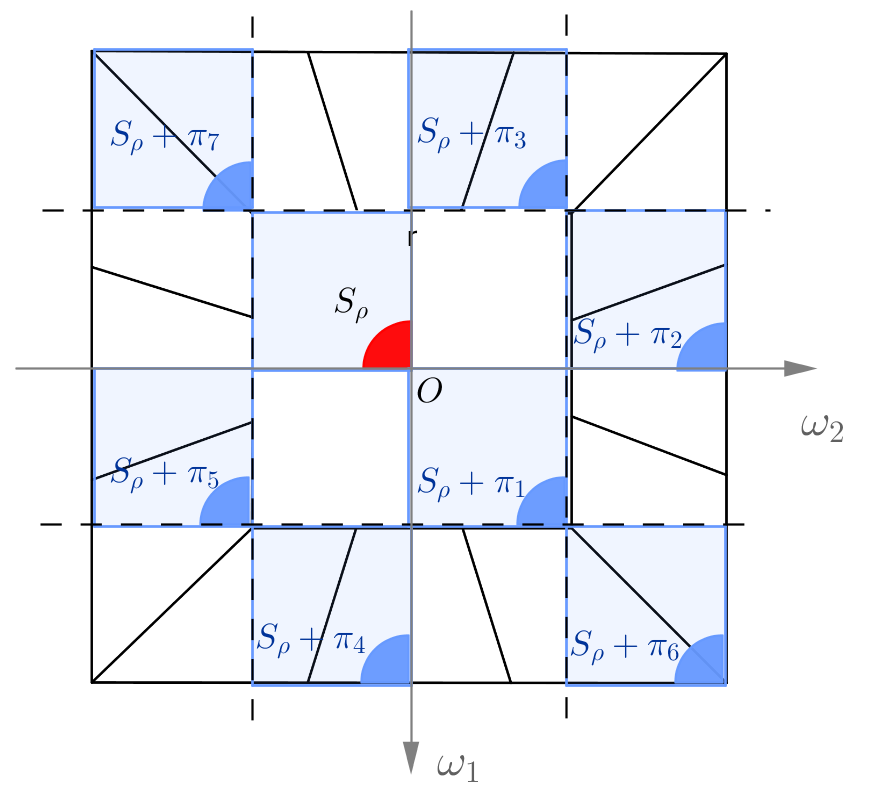
\includegraphics[width = .4\textwidth]{S_shifts2.png}
\caption{$S_{\rho}$ and its shifts}
\label{fig: S-shifts}
\end{figure}
Given directional selective $\m{i}$ that concentrates in $T_i$, we study the feasibility condition in Proposition \ref{prop: feasibility} specifically on the domain $S_{\rho} = \{(\omega_x,\omega_y)|\;\Vert\omega\Vert < \rho, \omega_x <0,\,\omega_y<0\}$. When $\rho$ is small enough, $\m{i}$ is zero on all but a few sets $S_\rho + \V{\pi}_j$ (see Fig.\ref{fig: S-shifts} for reference of $S_\rho$ and its shifts), thus $\mrow{i}(\V{\omega})$ is sparse on $S_\rho$ in the following form
\begin{align}
\label{eq: sparse-mat}
\begin{bmatrix}
\mrow{0}\\
\mrow{2}\\
\mrow{4}\\
\mrow{6}\\
\mrow{1}\\
\mrow{3}\\
\mrow{5}\\
\mrow{7}
\end{bmatrix}
=
\begin{bmatrix}
0 & 0 & 0 & 0 & 0 & 0\\
0 & * & * & 0 & 0 & 0\\
0 & 0 & 0 & * & * & 0\\
* & 0 & 0 & 0 & 0 & *\\
* & 0 & 0 & 0 & 0 & *\\
0 & 0 & * & * & 0 & 0\\
0 & 0 & * & * & 0 & 0\\
* & 0 & 0 & 0 & 0 & *
\end{bmatrix}
=\V{P}\,\widetilde{\mathbf{M}}[:,2:7],
\end{align}
where $\V{P}$ is a row permutation matrix. 
\begin{lemma}\label{lem: rank1}
$rank(\mrow{1},\mrow{7}) = 1$ in \eqref{eq: sparse-mat}.
\end{lemma}
\noindent{\it Proof.}
We make the following observation of $\mrow{i}$ in \eqref{eq: sparse-mat}:
\begin{itemize}
\item[(i)] $\mrow{0}$ is a zero vector
\item[(ii)] $\mrow{2}$ and $\mrow{4}$ are linearly independent of each other and the rest of $\mrow{i}$
\item[(iii)] $span\{\mrow{1},\mrow{6},\mrow{7}\} \perp span\{\mrow{3},\mrow{5}\}$ and $rank(\mrow{1},\mrow{6},\mrow{7}) \leq 2$, $rank(\mrow{3},\mrow{5})\leq 2$
\end{itemize}
Because $\widetilde{\mathbf{M}}[2:8,2:7]$ consists of rows $\mrow{i},\,i\neq 0$, and the low-pass function $m_0(\V{\omega})\neq 0,\, \forall\V{\omega}\in S_\rho$, or equivalently $rank(\widetilde{\mathbf{M}}[2:8,2:7](\V{\omega})) = 6$, it follows from  (ii) and (iii) that $rank(\mrow{1},\mrow{6},\mrow{7}) = 2$ and $rank(\mrow{3},\mrow{5})= 2$.\\
On the other hand, (ii) implies that $$rank(\widetilde{\mathbf{M}}[2:8,2:7](\V{\omega}+\V{\pi}_2))=rank(\mrow{4},\mrow{6},\mrow{1},\mrow{3},\mrow{5},\mrow{7})\leq 5$$ and $rank(\widetilde{\mathbf{M}}[2:8,2:7](\V{\omega}+\V{\pi}_4))=rank(\mrow{2},\mrow{6},\mrow{1},\mrow{3},\mrow{5},\mrow{7})\leq 5$ likewise. Therefore, $m_0(\V{\omega}+\V{\pi}_2) = m_0(\V{\omega}+\V{\pi}_4) = 0$.\\
If $\mrow{1}$ and $\mrow{7}$ are linearly independent, then $rank(\mrow{2},\mrow{4},\mrow{1},\mrow{3},\mrow{5},\mrow{7}) = 6$ and $m_0^C(\V{\omega}+\V{\pi}_6)\neq 0$, hence $m_0(\V{\omega}+\V{\pi}_6)\neq 0$. Therefore, $[m_0(\V{\omega}),m_0(\V{\omega}+\V{\pi}_2),m_0(\V{\omega}+\V{\pi}_4),m_0(\V{\omega}+\V{\pi}_6)] = [m_0(\V{\omega}),0,0,m_0(\V{\omega}+\V{\pi}_6)]$. In addition, $d_{i,j} = 0,\, \forall(i,j)$ except $(0,6)$, so $\mathfrak{D}(\V{\omega}) = [d_{0,6}, 0, 0,0]^\top [0,0,0,1] + [0,0,0,d_{0,6}]^\top [-1,0,0,0]$.  By Prop.\ref{prop: feasibility}, the linear system \eqref{eq: LS-new} has no solution $\forall \widetilde{m_0}$ and the lemma is proofed.\qed
\begin{lemma}\label{lem: concentrate}
If $\m{1} (\m{6})$ concentrates in $T_1 (T_6)$ and its essential support $\Omega_1\subset T_1 (\Omega_6\subset T_6)$, then $|\m{6}| > |\m{1}|\, a.e.$ on $T_6\bigcap \text{supp}(\widetilde{m_6})$ ($|\m{1}| > |\m{6}|\,a.e.$ on $T_1\bigcap\text{supp}(\widetilde{m_1})$).
\end{lemma}
\noindent{\it Proof}
Let $B_6=\{\V{\omega}: |\m{6}| \leq |\m{1}|, \m{1}\neq 0\}\bigcap T_6$ and $B_1$ be its mirror set with respect to $\omega_y = \omega_x$ and suppose $|B_6|>0$, then $\int_{B_6}|\m{6}|\leq \int_{B_6}|\m{1}|$. Since $\m{1}$ concentrates in $T_1$, we know $\int_{B_1}|\m{1}| > \int_{B_6}|\m{1}|$. On the other hand, due to the symmetry of $\m{1},\m{6}$ and $B_1,B_6$, $\int_{B_1}|\m{1}| = \int_{B_6}|\m{6}|$, hence $\int_{B_6}|\m{1}| \geq \int_{B_1}|\m{1}| $ which results in contradiction.\qed

\begin{proposition}
If  $m_1\,(m_6)$ concentrates within $T_1\,(T_6)$ and $\Omega_1\subset T_1\,(\Omega_6\subset T_6)$, then $\m{1} = \m{6} = 0,\, a.e. \,\V{\omega}\in S_\rho + \V{\pi}_1$.
\end{proposition}
\noindent{\it Proof.}
By Lemma \ref{lem: concentrate}, $|\m{1}| > |\m{6}|\, a.e.$ on $\Omega_1':= (S_\rho + \V{\pi}_7)\bigcap T_1 = (S_\rho+\V{\pi}_1)\bigcap T_6+(\pi,\pi)$. By Lemma \ref{lem: rank1}, $\exists\,\alpha_{\V{\omega}}\in\mathbb{C}, s.t.\,\mrow{1}(\V{\omega}) = \alpha_{\V{\omega}}\,\mrow{7}(\V{\omega})$, hence $|\widetilde{m_1}(\V{\omega})| = |\alpha_{\V{\omega}}|\cdot|\widetilde{m_1}(\V{\omega}-(\pi,\pi))| \geq |\alpha_{\V{\omega}}|\cdot|\widetilde{m_6}(\V{\omega}-(\pi,\pi))| = |\m{6}|, a.e. $ on $\Omega_6':= (S_\rho+\pi_1)\bigcap T_6$. Therefore, $\int_{\Omega_6'}|\widetilde{m_1}| \geq \int_{\Omega_6'}|\widetilde{m_6}|$, which will contradict Lemma \ref{lem: concentrate} unless $|\Omega_6'\bigcap\text{supp}(\widetilde{m_6})| = 0$, or equivalently $\alpha_{\V{\omega}}=0$ and so $\m{6} = \m{1} = 0,\,a.e.$ on $(S_\rho+\V{\pi}_1)\bigcap T_6$. By symmetry, $\m{6}=\m{1} = 0,\,a.e. $ on $(S_\rho+\V{\pi}_1)\bigcap T_1$ as well.\qed

\begin{proposition}
$\m{1},\m{3}$ are not continuous at $\V{\pi}_1,\V{\pi}_7$ and $\m{5},\m{7}$ are not continuous at $\V{\pi}_3,\V{\pi}_5$.
\end{proposition}
\noindent{\it Proof}
If $\m{1}$ is continuous at $\V{\pi}_1$, then $\widetilde{m_1}(\V{\pi}_1) = \lim_{\alpha\rightarrow 1^-}\widetilde{m_1}(\V{\omega}(\alpha)) = 0$, where $\{\V{\omega}(\alpha),\,0\leq \alpha<1\} \subset S_\rho + \V{\pi}_1$ and $\V{\omega}(1^-) = \V{\pi}_1$. Similarly, we have $\widetilde{m_6}(\V{\pi}_1) = 0$. Applying the same argument of $S_\rho$ to its rotation of 180 degree, we have $\widetilde{m_1}(\V{\pi}_7) = \widetilde{m_6}(\V{\pi}_7) = 0$. Therefore $\mrow{1}(0) = \mrow{7}(0) = \mathbf{0}$ and from \eqref{eq: m0C} $m_0^C(0)=0$ so that $m_0(0)=0$, %  On the other hand, Proposition\ref{prop: origin-det} implies that $m_0(0) = 0$ as $a = |\widetilde{m_1}(\pi_1)| = 0$,
 which results in contradiction.\qed\\[1em]
The following theorem summarizes the necessary condition derived from the singularity condition of $\M[2:8,:] $\eqref{eq: singular-cond}. 
\begin{theorem}\label{thm: thm}
If  $\m{i}$ concentrates in $T_i$ with essential support $\Omega_i\subset T_i$ and $m_1,m_6$ are symmetric to each other or $m_3,m_4$ are symmetric to each other,  then  \eqref{eq: LS-new} doesn't have feasible solution given continuous $\m{i}$.
\end{theorem}

\subsection{Design of input $\m{i}$}\label{sec: phase-design}
Following the orthonormal construction in \cite{yin2014orthshear}, we consider $\m{1},$ $\cdots,\m{6}$ in the form 
\begin{align}\label{eq: m-form}
\m{k} = e^{-i\eta_k^\top\omega}|\m{k}|,
\end{align}
 and $|\m{k}|$ have certain symmetry. We want to design the phase $\V{\eta}_k$ such that $m_0(\V{\omega}) > 0, \; \forall \omega\in S_1$. This is the same as requiring $\Msub$ to be full rank.
 We first show the necessary conditions on phases $\V{\eta}$ of the full rank requirement on $\Msub$.
 
\begin{lemma}
If $\exists\,\V{\omega}\in D_1:=\{\omega_x=\omega_y,\,\omega_x\in(-\frac{\pi}{2},0)\},\,s.t. \,m_0(\V{\omega})>0,$ then $(\V{\eta}_1-\V{\eta}_6)^\top (\V{\pi}_6-\V{\pi}_7)\neq 0(\text{mod}\,2\pi)$. 
\end{lemma} 
\noindent {\it Proof}
  If $m_0(\V{\omega})>0, \,\V{\omega}\in D_1$ then $\Msub$ is full rank, hence its columns are linearly independent. Due to symmetry, $|\widetilde{m_1}(\V{\omega})| = |\widetilde{m_6}(\V{\omega})|$ on $\{\omega_x=\omega_y\}$. Let $A = |\widetilde{m_1}(\V{\omega}+\V{\pi}_1)| = |\widetilde{m_6}(\V{\omega}+\V{\pi}_1)|$ and $B=|\widetilde{m_1}(\V{\omega}+\V{\pi}_6)| = |\widetilde{m_6}(\V{\omega}+\V{\pi}_6)|$, then the first and the last columns of $\Msub$ are
  \begin{align*}
  \Msub[:,1] = 
 \begin{bmatrix}
 0\\
 \vdots\\
 0\\
 Ae^{i\V{\eta}_1^\top(\V{\omega}+\V{\pi}_6)}\\
 Be^{i\V{\eta}_1^\top(\V{\omega}+\V{\pi}_7)}
 \end{bmatrix}
 \quad\text{and}\quad
  \Msub[:,6] = 
 \begin{bmatrix}
 0\\
 \vdots\\
 0\\
 Ae^{i\V{\eta}_6^\top(\V{\omega}+\V{\pi}_6)}\\
 Be^{i\V{\eta}_6^\top(\V{\omega}+\V{\pi}_7)}
 \end{bmatrix} .
\end{align*}   
Therefore, $\Msub[:,1]$ and $\Msub[:,6]$ are linearly independent implies that $e^{i(\V{\eta}_1-\V{\eta}_6)^\top(\V{\omega}+\V{\pi}_6)}\neq e^{i(\V{\eta}_1-\V{\eta}_6)^\top(\V{\omega}+\V{\pi}_7)}$ or equivalently $(\V{\eta}_1-\V{\eta}_6)^\top(\V{\pi}_6-\V{\pi}_7)\neq 0(\text{mod}2\pi)$. \qed\\

Similarly, if $\exists\,\V{\omega}\in \{\omega_y = \omega_x,\, \omega_x\in(0,\frac{\pi}{2})\},\, s.t.\, m_0(\V{\omega}) > 0$, then $(\V{\eta}_1-\V{\eta}_6)^\top (\V{\pi}_6-\V{\pi}_1)\neq 0(\text{mod}\,2\pi)$. These two conditions are equivalent to 
\begin{align*}
(\V{\eta}_1-\V{\eta}_6)^\top(\pi/2,\pi/2)\neq 0 (\text{mod}\,2\pi)\tag{\bf c1.1}
\end{align*}
given that $\V{\eta}_1$ and $\V{\eta}_6$ are integer phases.
A stronger condition is to require $\Msub[:,1]$ and $\Msub[:,6]$ be orthogonal, which is equivalent to 
\begin{align*}
(\V{\eta}_1-\V{\eta}_6)^\top(\pi/2, \pi/2) = \pi \,(\text{mod}\, 2\pi).\tag{\bf c2.1}
\end{align*}
Considering the other diagonal segment $\{\omega_y = -\omega_x, |\omega_x| <\frac{\pi}{2}\}$, we have 
\begin{align*}
(\V{\eta}_3-\V{\eta}_4)^\top(-\pi/2,\pi/2)\neq 0 (\text{mod}\, 2\pi)\tag{\bf c1.2}
\end{align*}
from the full rank condition and 
\begin{align*}
(\V{\eta}_3-\V{\eta}_4)^\top(-\pi/2,\pi/2)=\pi(\text{mod},\,2\pi)\tag{\bf c2.2}
\end{align*} from the stronger orthogonal condition.
{\it Remark}
If $|\m{1}| = |\m{2}|$ on $\{\omega_y = 3\omega_x,\,|\omega_x| > \frac{\pi}{2}\}$ and $m_0(\V{\omega}) > 0$ on $\{\omega_y = 3\omega_x\pm \pi,\,|\omega_y| <\frac{\pi}{2}\}$, then the same conditions ({\bf c1}) and ({\bf c2}) can be derived from full rank and orthogonal conditions respectively for tuples $(\,\V{\eta}_1,\,\V{\eta}_2,(-\pi/2,\pi/2)\,),\,(\,\V{\eta}_2,\V{\eta}_3,(\pi/2,\pi/2)\,),\,(\V{\eta}_4,\V{\eta}_5,\,(\pi/2,\pi/2)\,)$ and $(\,\V{\eta}_5,\V{\eta}_6,\,(-\pi/2,\pi/2)\,)$. 

Next, we investigate $\Msub$ at the origin, where the two diagonals meet.
\begin{proposition}\label{prop: origin-det}
If $m_0(0) > 0,$ then $\V{\pi}_1^\top(\V{\eta}_1-\V{\eta}_6)\neq \pi(\text{mod}\,2\pi)$ or $\V{\pi}_3^\top(\V{\eta}_3-\V{\eta}_4)\neq \pi(\text{mod}\,2\pi)$. 
\end{proposition}
\noindent{\it Proof}
$\Msub(0)$ takes the following form
$$\begin{bmatrix}
* & 0 & 0 & 0 & 0 & *\\
0 & * & 0 & 0 & 0 & 0\\
0 & 0 & * & * & 0 & 0\\
0 & 0 & 0 & 0 & * & 0\\
0 & 0 & * & * & 0 & 0\\
* & 0 & * & * & 0 & *\\
* & 0 & 0 & 0 & 0 & *
\end{bmatrix}$$
The second and the fifth columns of $\Msub$ have single non-zero entry, $\widetilde{m_2}(\V{\pi}_2)$ and $\widetilde{m_5}(\V{\pi}_4)$ respectively, and are orthogonal to all the rest columns, hence the full-rank constraint of $\Msub$ is reduced to the full-rank constraint on its sub-matrix (with permutation of rows and columns)
$$ \overline{\mbox{B\strut}} := \overline{\Msub}[-2,-4,:]=
\begin{bmatrix}
& & & \\[-1em]
\widetilde{m_1}(\V{\pi}_6) & \widetilde{m_6}(\V{\pi}_6) & \widetilde{m_3}(\V{\pi}_6) & \widetilde{m_4}(\V{\pi}_6) \\
\widetilde{m_1}(\V{\pi}_1) & \widetilde{m_6}(\V{\pi}_1) & 0 & 0\\
\widetilde{m_1}(\V{\pi}_7) & \widetilde{m_6}(\V{\pi}_7) & 0 & 0\\
0 & 0 & \widetilde{m_3}(\V{\pi}_3) & \widetilde{m_4}(\V{\pi}_3)\\
0 & 0 & \widetilde{m_3}(\V{\pi}_5) & \widetilde{m_4}(\V{\pi}_5)\\
\end{bmatrix}
$$
Without loss of generality, let $|\widetilde{m_1}(\V{\pi}_1)| = |\widetilde{m_1}(\V{\pi}_7)| = |\widetilde{m_6}(\V{\pi}_1)| = |\widetilde{m_6}(\V{\pi}_7)| = |\widetilde{m_3}(\V{\pi}_3)| = |\widetilde{m_3}(\V{\pi}_5)| = |\widetilde{m_4}(\V{\pi}_3)| = |\widetilde{m_4}(\V{\pi}_5)|= a$ and $|\widetilde{m_1}(\V{\pi}_6)|=| \widetilde{m_6}(\V{\pi}_6)|= | \widetilde{m_3}(\V{\pi}_6)|=| \widetilde{m_4}(\V{\pi}_6)|=b$. Rewrite $\overline{\mbox{B\strut}}$ as follows,
$$\overline{\mbox{B\strut}}=
\begin{bmatrix}
b e^{-i\V{\pi}_6^\top\V{\eta}_1} & b e^{-i\V{\pi}_6^\top\V{\eta}_6} & b e^{-i\V{\pi}_6^\top\V{\eta}_3} & b e^{-i\V{\pi}_6^\top\V{\eta}_4}\\
a e^{-i\V{\pi}_1^\top\V{\eta}_1} & a e^{-i\V{\pi}_1^\top\V{\eta}_6} & 0						& 0 \\
a e^{i\V{\pi}_1^\top\V{\eta}_1} & a e^{i\V{\pi}_1^\top\V{\eta}_6} & 0						& 0 \\
0 					& 0 					& a e^{-i\V{\pi}_3^\top\V{\eta}_3} & a e^{-i\V{\pi}_3^\top\V{\eta}_4}\\
0 					& 0 					& a e^{i\V{\pi}_3^\top\V{\eta}_3} & a e^{i\V{\pi}_3^\top\V{\eta}_4}\\
\end{bmatrix}
$$
The product of singular values of $\V{B}$ is 
\begin{align}\label{eq: detB}
\sqrt{\text{det}(\V{B}^* \V{B})} = 4a^3\sqrt{a^2 K_1^2K_2^2 + b^2(Q_1K_2^2 + Q_2K_1^2)},
\end{align}
where $ Q_1 = 1 - \cos(\V{\pi}_6^\top(\V{\eta}_1-\V{\eta}_6))\cos(\V{\pi}_1^\top(\V{\eta}_1-\V{\eta}_6)), Q_2 = 1 - \cos(\V{\pi}_6^\top(\V{\eta}_3-\V{\eta}_4))\cos(\V{\pi}_3^\top(\V{\eta}_3-\V{\eta}_4)), K_1 = \sin(\V{\pi}_1^\top(\V{\eta}_1-\V{\eta}_6)), K_2 = \sin(\V{\pi}_3^\top(\V{\eta}_3-\V{\eta}_4)).$

 If the previous strong orthogonal condition on $\V{\eta}_1, \V{\eta}_3, \V{\eta}_4,\V{\eta}_6$ holds, then $K_1 = K_2 = 0$ and $m_0(0)=m_0^C(0)= 0$. Therefore, the strong orthogonal condition ({\bf c2}) cannot be satisfied at the same time. 
In particular, we consider the following constraints on phase $\V{\eta}_k\in \mathbb{Z}^2,\, k = 1,\cdots,6$:
\begin{align}
\label{eq: phase-constraint}
&(\V{\eta}_1-\V{\eta}_2)^\top(-\pi/2, \pi/2) = (\V{\eta}_5-\V{\eta}_6)^\top(-\pi/2,\pi/2) = \pi\, (\text{mod}\, 2\pi)\notag\\
&(\V{\eta}_2-\V{\eta}_3)^\top(\pi/2,\pi/2) = (\V{\eta}_4-\V{\eta}_5)^\top(\pi/2,\pi/2) = \pi\, (\text{mod}\, 2\pi)\\
&(\V{\eta}_3-\V{\eta}_4)^\top(-\pi/2, \pi/2) =-\pi/2\,(\text{mod}\,2\pi)\quad (\V{\eta}_6 - \V{\eta}_1)^\top(\pi/2,\pi/2) = \pi/2\, (\text{mod}\,2\pi) \notag
\end{align}
where we require strong orthogonal constraints on pair of shifts corresponding to $\widetilde{m}$ function with non-diagonal common boundary and weaker constraints on $(\V{\eta}_1,\V{\eta}_6)$ and $(\V{\eta}_3,\V{\eta}_4)$. A solution to \eqref{eq: phase-constraint} is 
\begin{align}\label{eq: phase-sol}
\V{\eta}_1 = (0,0),\; \V{\eta}_2 = (-1,1),\; \V{\eta}_3 = (0,2),\notag\\
\V{\eta}_4 = (1,0),\; \V{\eta}_5 = (0,-1),\; \V{\eta}_6 = (0,1).
\end{align}

\subsection{solving $m_i$}
In the final step, we substitute $\mc{0}$ and $m_0^C(\V{\omega})$ into \eqref{eq: LS-new} and rewrite it into the following linear system,
\begin{align}\label{eq: mi}
\overline{\M}[:,2:7]\,\mathbf{m}[2:7](\V{\omega}) = 
\begin{bmatrix}
1-m_0^C\overline{\widetilde{m_0}^C}(\V{\omega})\\
0\\
-m_0^C\overline{\widetilde{m_0}^C}(\V{\omega}+\V{\pi}_2)\\
\vdots \\
0
\end{bmatrix}
=:\mathbf{b}(\V{\omega}).
\end{align}
The solution of \eqref{eq: mi} depends only on $m_0^C\overline{\widetilde{m_0}^C}$, or equivalently $m_0\overline{\widetilde{m_0}}$. 


\section{Numerical Experiments}
\subsection{solving $m_0^C$}
A set of $\m{i}$ that satisfy the conditions of Theorem \ref{thm: thm} with phase terms in \eqref{eq: phase-sol} is used as the input of \eqref{eq: LS-new}.
The left figure in Fig.\ref{fig: tm_i_m_0} shows the absolute value of $\m{i}$. In particular, $\m{i} =0,\,\forall \omega\in S_1$. 
We follow the construction process in Section \ref{subsec: compute-m0} and obtain $m_0^C$ shown in the right of Fig.\ref{fig: tm_i_m_0}, in both normal scale and log scale.  
We perform a numerical sanity check on the necessary condition in Proposition \ref{prop: feasibility}, that is $\forall\,\V{\omega}, \,s.t. [m_0(\V{\omega}), m_0(\V{\omega}+\V{\pi}_2),m_0(\V{\omega}+\V{\pi}_4),m_0(\V{\omega}+\V{\pi}_6)]$ is not a linear combination of the rows of $\mathfrak{D}(\V{\omega})$ in \eqref{eq: singular-cond}. Equivalently, we compute the following quantity $$\vartheta = 1 - \Vert V^\top\mathfrak{m}_0 \Vert/\Vert \mathfrak{m}_0\Vert ,$$ where $\mathfrak{m}_0(\V{\omega})=[m_0(\V{\omega}), m_0(\V{\omega}+\V{\pi}_2),m_0(\V{\omega}+\V{\pi}_4),m_0(\V{\omega}+\V{\pi}_6)]^\top$ and $V$ are the left singular vectors of $\mathfrak{D}(\omega)$ whose corresponding singular values are non-zero. If $\mathfrak{m}_0\in span(V)$, then $\vartheta = 0$. If $\mathfrak{m}_0\bot span(V)$, then $\vartheta = 1$.
Fig.\ref{fig: feasible} shows the feasibility check $\vartheta$ of input $\m{i}$, and $\mathfrak{m}_0$ is orthogonal to $span(V)$ everywhere.

\begin{figure}
\centering
\begin{minipage}[c]{.48\textwidth}
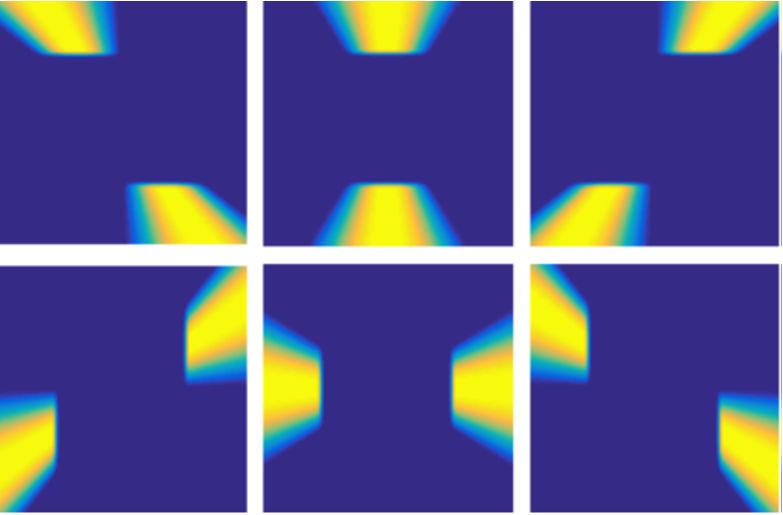
\includegraphics[width=\textwidth]{feasible_mi.pdf}
\end{minipage}
\begin{minipage}[c]{.22\textwidth}
\centering
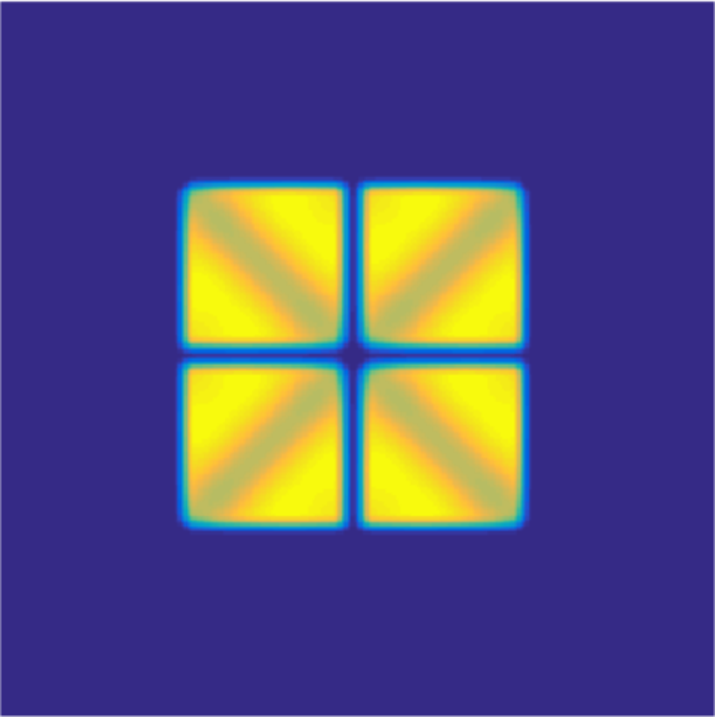
\includegraphics[width=.8\textwidth]{feasible_m0.pdf}
\end{minipage}
\begin{minipage}[c]{.28\textwidth}
\centering
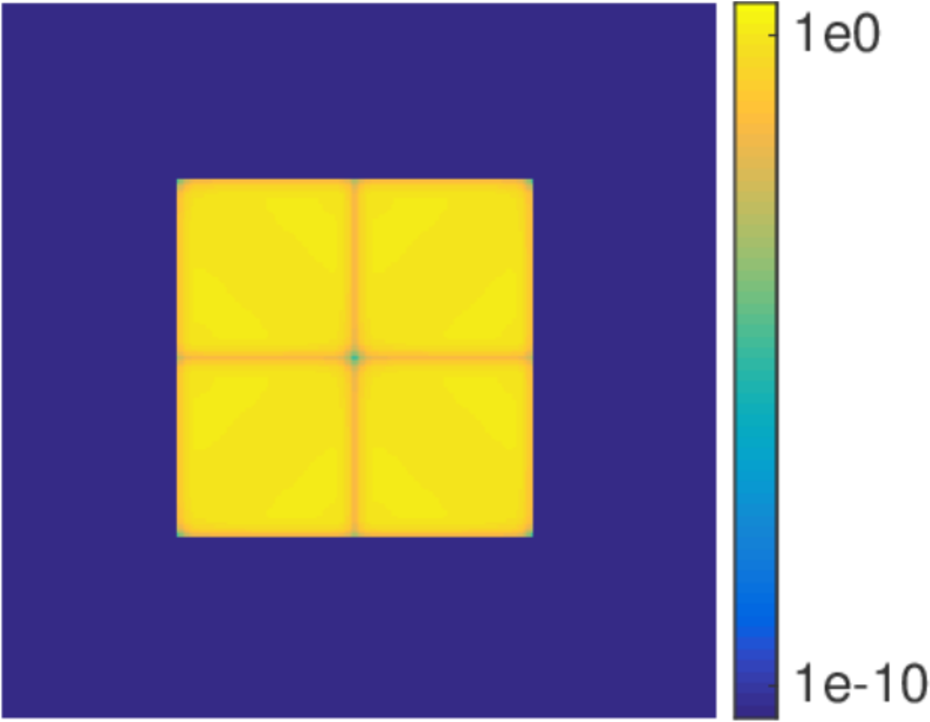
\includegraphics[width=.8\textwidth]{feasible_m0_log.pdf}
\end{minipage}
\caption{Left:  $|\m{i}|$, middle: computed $m_0^C$, right: $\log(m_0^C)$}
\label{fig: tm_i_m_0}
\end{figure}

\subsection{solving $\mc{0}$ and $m_i$}
We compute $\mc{0}$ by solving the following optimization problem similar to \eqref{eq: opt-diff} for the dyadic scheme,
\begin{align}
\min_{\xvec}\; \Vert \V{D}(\mathbf{m}_0^C\circ\xvec)\Vert^2 + \lambda\Vert \wvec\circ\mathbf{m}_0^C\circ\xvec\Vert^2,\quad 
s.t. \; A\xvec = \mathbf{1},\, \mathfrak{D}\xvec = \mathbf{0}
\label{eq: opt-2d}
\end{align}
where $\circ$ is Hadamard product and $\wvec$ is a weight vector and we consider real solution $\xvec$ here.
$A$ in the constraint is the matrix generated from the identity condition \eqref{eq: identity-cond} and $\mathfrak{D}$ is generated from the singularity condition \eqref{eq: singular-cond}. Since $A$ and $\mathfrak{D}$ are linearly independent, \eqref{eq: opt-2d} is feasible. Here, instead of optimizing the properties of $\xvec$ as in \eqref{eq: opt-diff}, we optimize those of $\widetilde{\mathbf{m}_0}^C\circ \xvec$ since $m_0^C \cdot\widetilde{m_0}^C$ will be later re-decomposed into $m_0$ and $\widetilde{m_0}$. In addition, if $m_0^C$ is symmetric with respect to the two coordinates $\omega_x$ and $\omega_y$, then we impose the same symmetry on $\widetilde{m_0}^C$ by solving \eqref{eq: opt-2d} on $[0,\pi)\times[0,\pi)$ and then extend the solution to $[-\pi,\pi)\times[-\pi,\pi)$ by symmetry.

\begin{figure}
\centering
\begin{minipage}[c]{.3\textwidth}
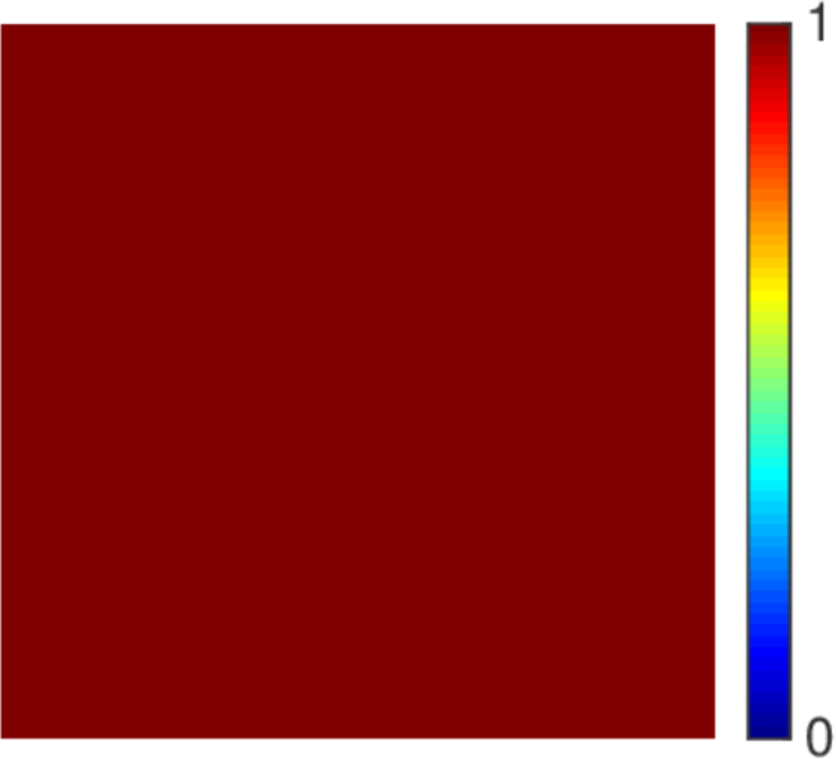
\includegraphics[width = .8\textwidth]{feasible_check.pdf}
\caption{$\vartheta$}\label{fig: feasible}
\end{minipage}
\begin{minipage}[c]{.63\textwidth}%{.28\textwidth}
\centering
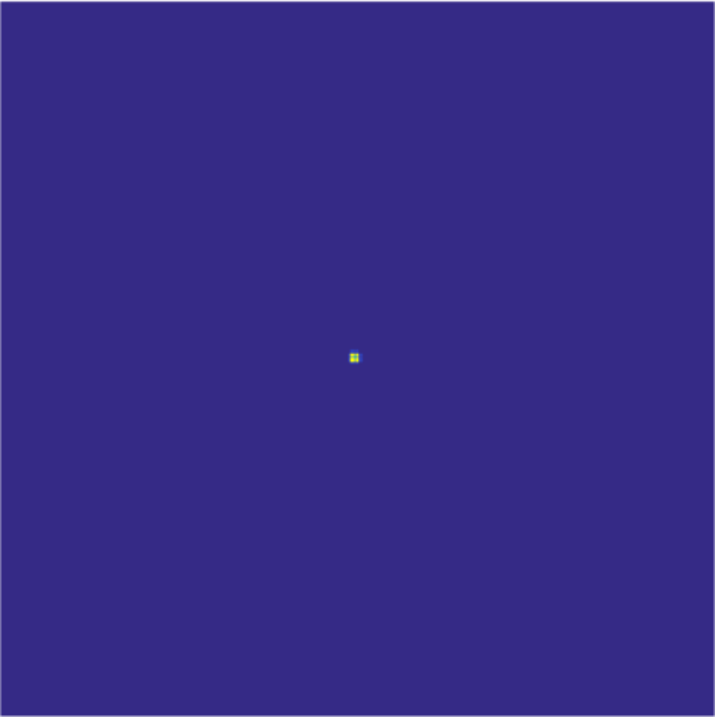
\includegraphics[width = .38\textwidth]{feasible_tm0.pdf}\hspace*{2em}
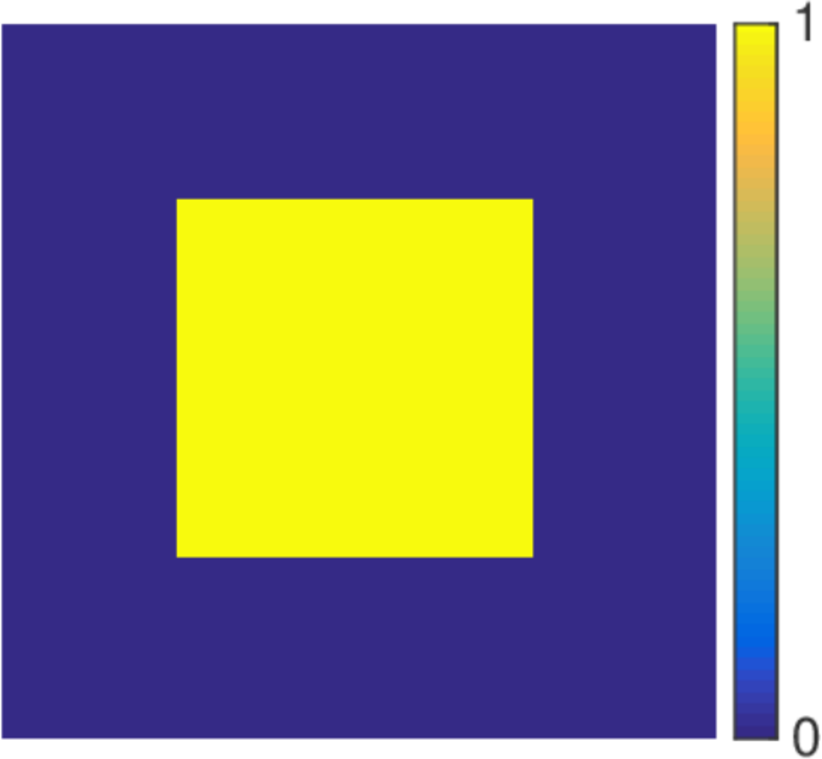
\includegraphics[width = .42\textwidth]{feasible_m0tm0.pdf}
\caption{Left: : computed $\widetilde{m_0}^C$, right: $\widetilde{m_0}^C \cdot m_0^C $}
\label{fig: tm0}
\end{minipage}
\end{figure}

Fig.\ref{fig: tm0} shows $\mc{0}$ obtained from \eqref{eq: opt-2d} and $\widetilde{m_0}^C \cdot m_0^C$ which is $\mathbf{1}_{S_1}$.

In particular, given $\widetilde{m_0}^C \cdot m_0^C = 1$, $\mathbf{b}(\V{\omega}) = \mathbf{0}, \, \forall\,\V{\omega}\in S_1$, hence $\mathbf{m}[2:7] = \mathbf{0}$. 
When $\mathbf{b}(\V{\omega})\neq \mathbf{0}$, \eqref{eq: mi} is a degenerated over-determinant linear system (we also do a sanity check here for the linearity between $\overline{\M}[:,2:7]$ and $\mathbf{b}$ by computing $\vartheta$) and 
$$\mathbf{m}[2:7](\V{\omega}) = \Big(\overline{\M}[:,2:7]\Big)^\dagger\,\mathbf{b}(\V{\omega}),$$
where $\dagger$ is the pseudo-inverse of a matrix. Fig.\ref{fig: m_i} shows the solution $m_i$ of \eqref{eq: mi} and the corresponding spatial filters $\mathcal{F}^{-1}\widetilde{m_0}$.
As shown in Fig.\ref{fig: m_i}, the energy of $m_i$ concentrates on $\{|\omega_x| = \frac{\pi}{2},\, |\omega_y| = \frac{\pi}{2}\}$ where $|\widetilde{m_i}|$ is small, and the filters decay slowly in time domain.

The bi-orthogonal bases constructed is not ideal, despite the regularization on $m_0$ in the optimization \eqref{eq: opt-2d}. Since no explicit regularization is put on $m_i$, it's difficult to control the regularity of the output $m_i$ from the input $\widetilde{m_i}$.

\begin{figure}
\centering
\begin{minipage}[c]{.5\textwidth}
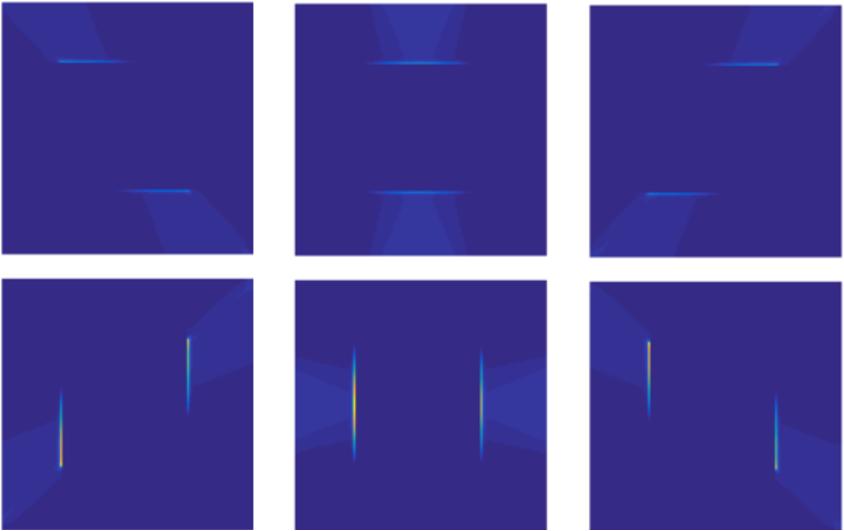
\includegraphics[width = .9\textwidth]{feasible_m.pdf}
\end{minipage}
\begin{minipage}[c]{.48\textwidth}
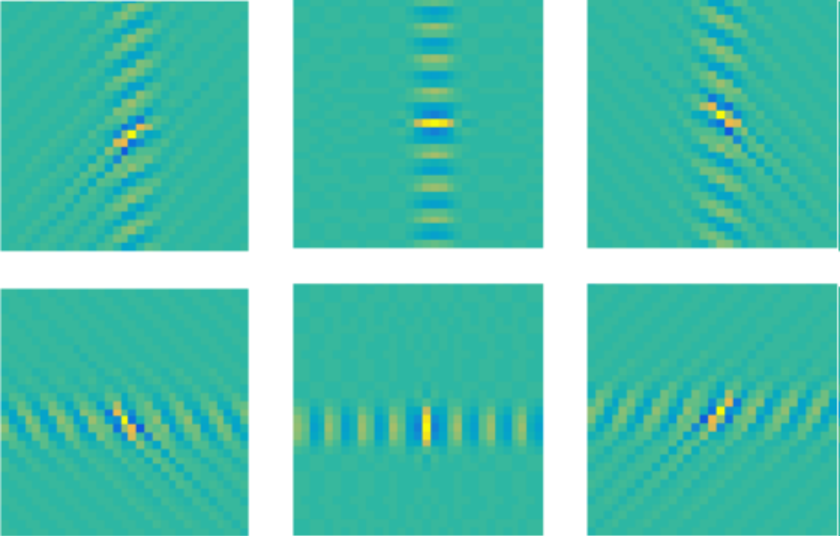
\includegraphics[width = .9\textwidth]{feasible_mi_time.pdf}
\end{minipage}
\caption{Left: $|m_i|,\, i = 1,\cdots,6$, right:$|\mathcal{F}^{-1}m_i|$}
\label{fig: m_i}
\end{figure}